\appendix

\chapter{Appendix}

\section{Small vs Large Vocabulary}\label{app:small_vs_large_vocabulary}

Some initial experiments were conducted over a smaller vocabulary with $C=26$. This vocabulary includes a symbol for major and minor over each root and two special symbols, \texttt{N} and \texttt{X} for no chord and unknown chord respectively. This contrasts the much larger vocabulary with 14 chord qualities for each root which is used for the majority of the experiments. With this larger vocabulary, $C=170$.

Table~\ref{tab:small_vs_large_vocab} shows the results of the \emph{CRNN} trained over the smaller and larger vocabulary evaluated on the small vocabulary. The predictions of the model and the reference labels are all mapped to the small vocabulary before being evaluated in the same was as described in Section~\ref{sec:evaluation}. This test was to verify that the model trained on the larger vocabulary performs well competitively on the smaller vocabulary. If the model trained on the larger vocabulary performed poorly on the smaller vocabulary, it may be prudent to first try to improve performance on this smaller vocabulary. It may also be a sign that the larger vocabulary is too complex or that the more detailed annotations are inconsistent.

However, the table shows very similar performance between both models. This allows us to proceed with the larger vocabulary for the rest of the experiments. The larger vocabulary is also more consistent with the literature and allows for a model to produce far more interesting chord predictions than simply minor, major and root. 

\begin{table}[H]
    \centering
    \begin{tabular}{lccc}
        \toprule
        Vocab & $C$ & acc & root \\  
        \midrule
        small & $26$ & 76.7 & 80.1 \\
        large & $170$ & 76.0 & 79.1 \\
        \bottomrule
    \end{tabular}
    \caption{\emph{CRNN} with a small and large vocabulary.}\label{tab:small_vs_large_vocab}
\end{table}

Note that the \texttt{mir\_eval} package also includes a \texttt{majmin} evaluation metric that compares chords over just the major and minor qualities. However, this is not quite the same as the test above due to subtleties in how \texttt{mir\_eval} chooses whether or not a chord is major or minor. It ends up ignoring many chords that could be mapped to these qualities in the smaller vocabulary. Coincidentally, \emph{CRNN} with the default parameters attains a \texttt{majmin} accuracy of $76.0\%$ over the larger vocabulary. This further confirms that we need not continue to test on the smaller vocabulary. The  \texttt{majmin} metric is not used in the rest of the thesis as it is not as informative as the other metrics and the \texttt{third} metric is highly correlated with it.

\section{Chord Mapping}\label{app:chord_mapping}

Chords in Harte notation were mapped to the vocabulary with $C=170$ by first converting them to a tuple of integers using the Harte library. These integers represent pitch classes and are in the range 0 to 11 inclusive. They are transposed such that 0 is the root pitch. These pitch classes were then matched to the pitch classes of a quality in the vocabulary, similar to the work by \citet{StructuredTraining}. However, for some chords, this was not sufficient. For example, a \texttt{C:maj6(9)} chord would not fit perfectly with any of these templates due to the added 9th. Therefore, the chord was also passed through Music21's~\citep{music21} chord quality function which matches chords such as the one above to major. This function would not work alone as its list of qualities is not as rich as the one defined above. If the chord was still not matched, it was mapped to \texttt{X}. This additional step is not done by \citet{StructuredTraining} but gives more meaningful labels to roughly one third of the chords previously mapped to \texttt{X}.

\section{CRNN with CR2}\label{app:crnn_with_cr2}

\begin{table}[H]
    \centering
    \begin{tabular}{lccccccc}
        \toprule
        cr2 & acc & root & third & seventh & mirex & acc\textsubscript{class} & median\textsubscript{class} \\  
        \midrule
        on & 59.7 & \textbf{78.9} & \textbf{75.6} & 61.9 & \textbf{80.5} & 18.4 & 0.4 \\
        off & \textbf{60.2} & 78.4 & 75.3 & \textbf{62.5} & 79.5 & \textbf{19.4} & \textbf{1.1} \\
        \bottomrule
    \end{tabular}
    \caption{\emph{CRNN} with and without the added `CR2' decoder. Performance is very similar between the two. It could be argued that te model with CR2 on is better, but for simplicity, I proceed with the model without CR2. One could also argue that the effect of CR2 is similar to simply adding more layers to the GRU already present in \emph{CRNN}.}
\end{table}

\section{A Long Run with SGD}\label{app:long_sgd}
\begin{figure}[H]
    \centering
    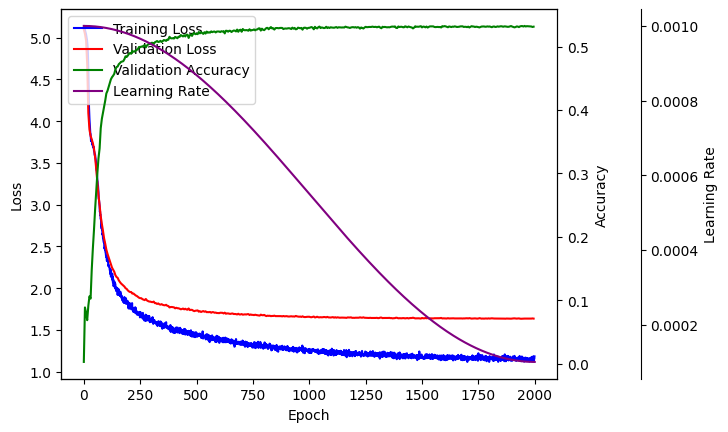
\includegraphics[width=1.0\textwidth]{figures/long_sgd_training_plot.png}
    \caption{Training graphs for \emph{CRNN} trained with SGD, momentum 0.9, a learning rate of $0.001$ and the \texttt{cosine} scheduling for 2000 epochs. Convergence is reached but performance does not exceed that which is achieved by Adam over 150 epochs. Furthermore, there is signifcant computational cost associated with running for 2000 epochs. I proceed with Adam for the remainder of experiments. }\label{fig:long_sgd}
\end{figure}


\section{Random Hyperparameter Search Sets}\label{app:random_hyperparameter_search_sets}

The hyperparameter search for \emph{CRNN} was done over the following variables and values:
\begin{itemize}
    \item \texttt{hidden\_size} $\in$ \{32, 64, 128, 256, 512\}
    \item \texttt{num\_layers} $\in$ \{1, 2, 3\}
    \item \texttt{segment\_length} $\in$ \{5, 10, 15, 20, 25, 30, 35, 40, 45\}
    \item \texttt{kernel\_size} $\in$ \{5, 6, 7, 8, 9, 10, 11, 12, 13, 14, 15\}
    \item \texttt{cnn\_layers} $\in$ \{1,2,\ldots,5\}
    \item \texttt{cnn\_channels} $\in$ \{1,2,\ldots,5\}
\end{itemize}

For each run, a value was selected for each hyperparameter, with each possible value equally likely.

% \section{CNN Hyperparameter Search}\label{app:cnn_hparams}

% \begin{table}[H]
%     \centering
%     \begin{tabular}{@{}cccccccccc@{}}
%         \toprule
%         $k$ & $l$ & $c$ & acc & root & third & seventh & mirex & acc\textsubscript{class} & median\textsubscript{class} \\  
%         \midrule
%         5 & 1 & 1 & 54.5 & 74.4 & 69.0 & 56.6 & 73.5 & 16.0 & 2.3 \\
%         5 & 3 & 5 & 57.0 & 76.9 & 72.5 & 59.2 & 77.6 & 18.9 & 3.0 \\
%         9 & 5 & 10 & \textbf{57.8} & \textbf{78.1} & \textbf{74.0} & \textbf{60.0} & \textbf{77.8} & \textbf{19.2} & \textbf{3.2} \\
%         \bottomrule
%     \end{tabular}
%     \caption{CNN hyperparameter search results. The best performing result for each metric is highlighted in \textbf{bold}. Performance increases with depth of the model. However, the performance increase is not significant between the two best performing models. Deeper CNNs were also trained, but were results did not improve and were too computationally intensive to run repeatedly.}
% \end{table}

\section{Confusion Matrix of CRNN over Roots}\label{app:cm_roots}

\begin{figure}[H]
    \centering
    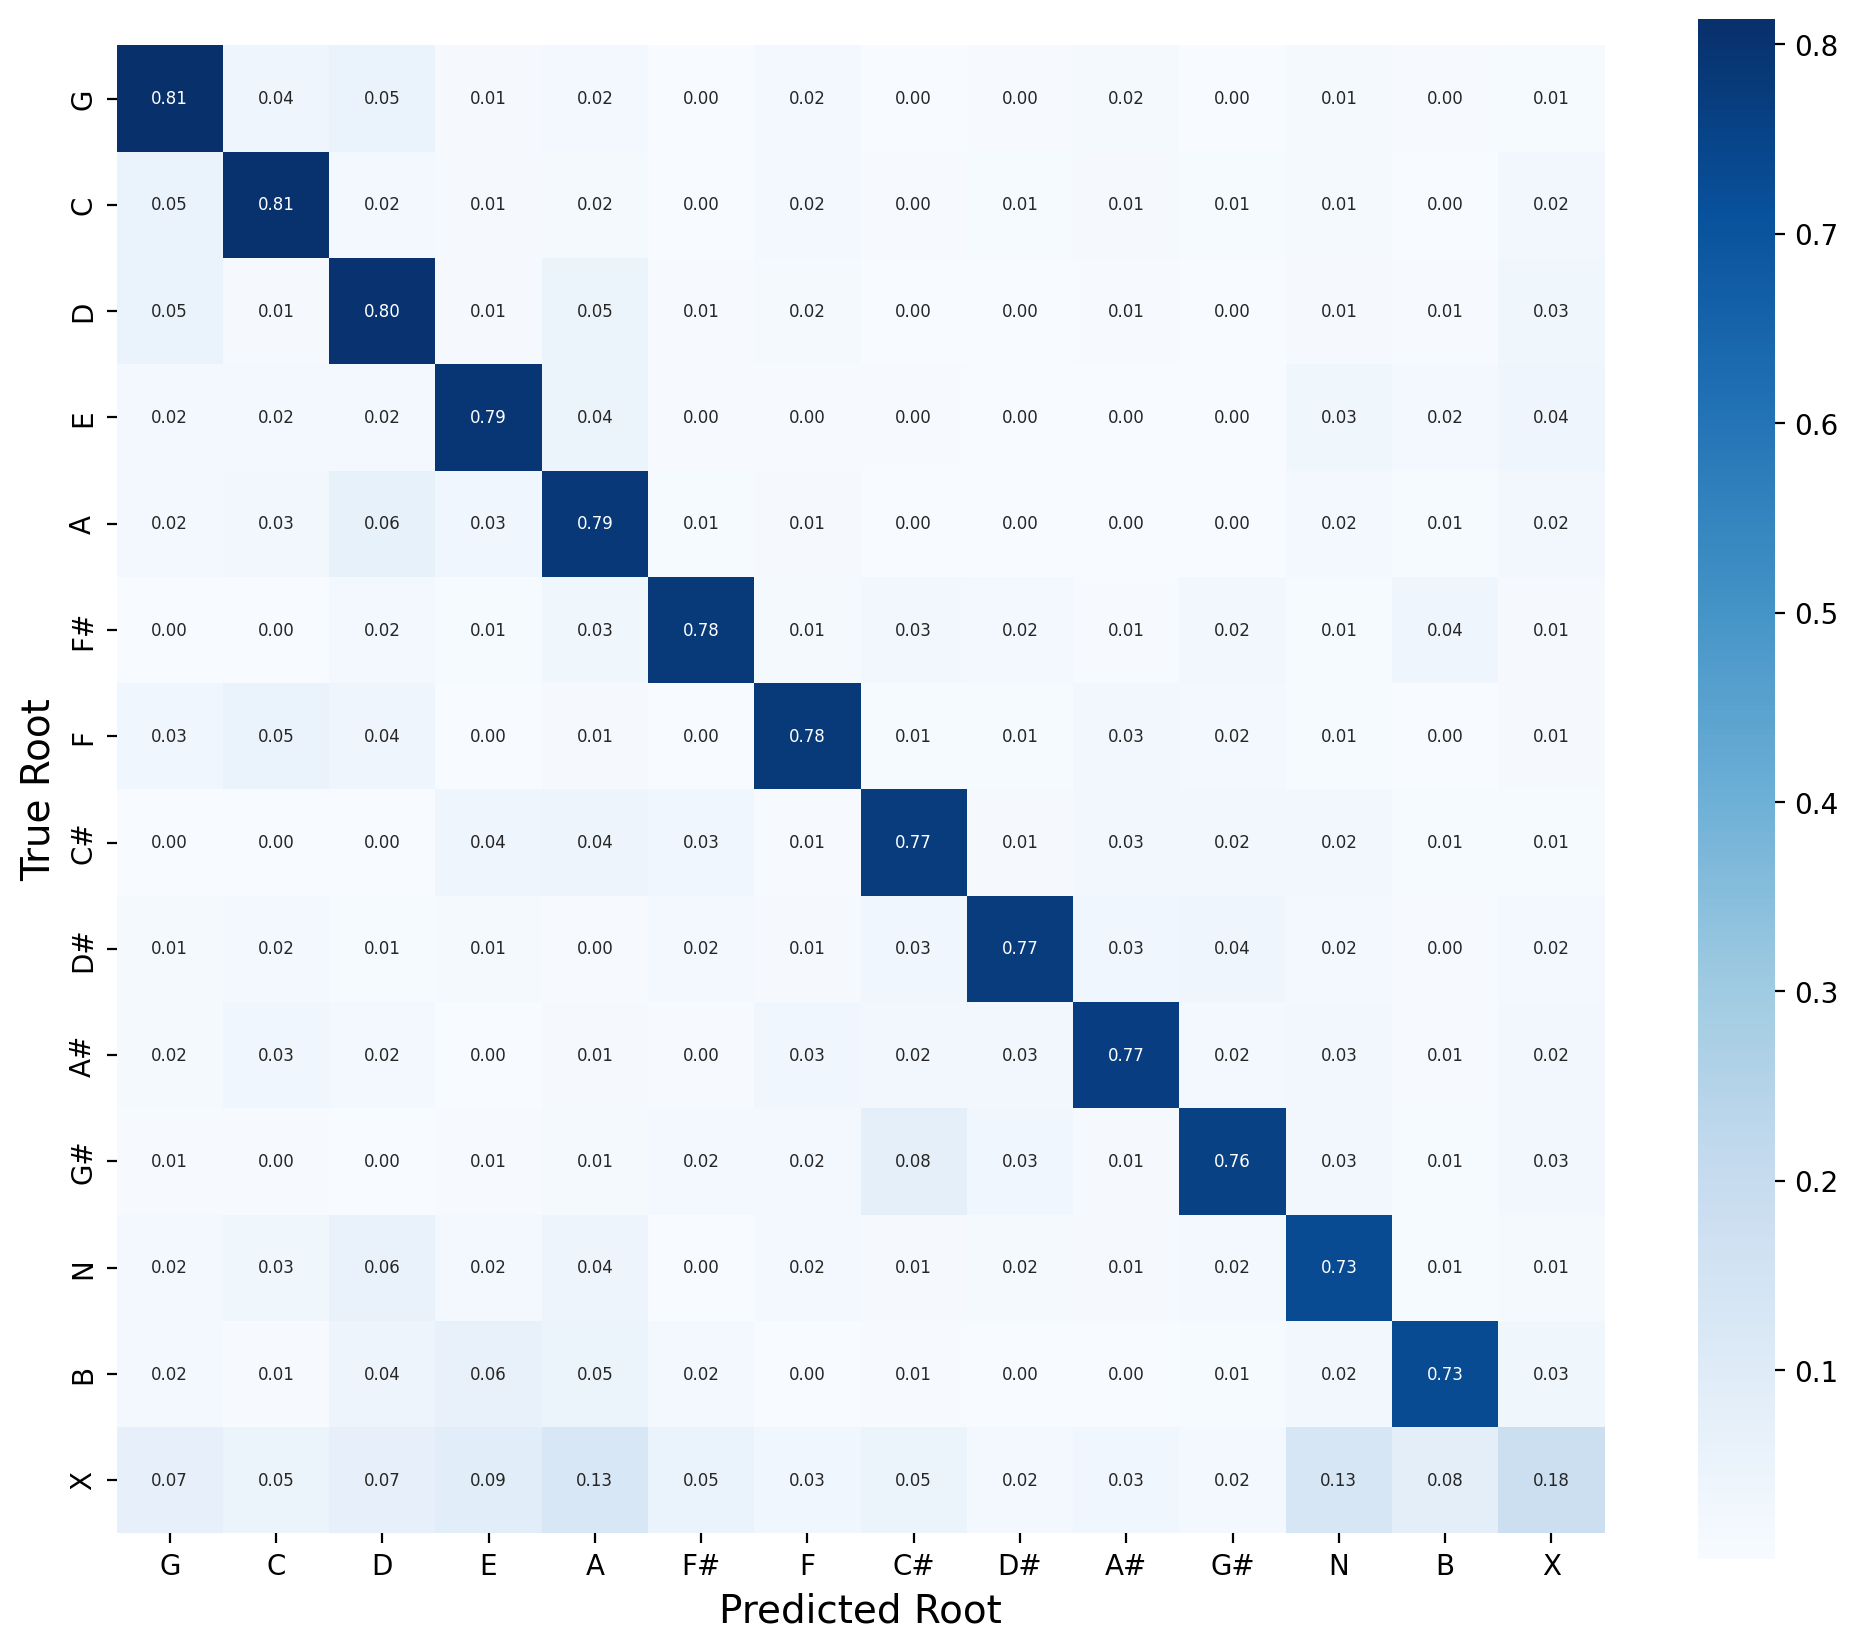
\includegraphics[width=1.0\textwidth]{figures/confusion_matrix_roots.png}
    \caption{Performance is relatively stable across roots. The only outlier is the unknown chord symbol \texttt{X}. This is to bexpected given the ambiguous nature of the chord. }
    \label{fig:cm_roots}
\end{figure}

% \section{Accuracy vs Hop Length}\label{app:accuracy_vs_hop_length}

% \begin{figure}[H]
%     \centering
%     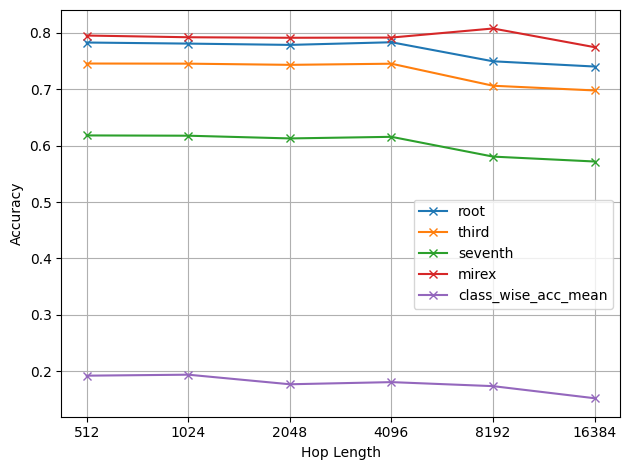
\includegraphics[width=0.5\textwidth]{figures/hop_length_vs_accuracy.png}
%     \caption{Accuracy vs hop length. Metrics are not directly comparable over hop lengths due to different likelihoods. However, the metrics are fairly consistent over different hop lengths, certainly over the region explored by the literature $[512,2048,4096]$. Every hop length tested is short enough to be more granular than chords, but not so short that the computed CQT is too noisy. We continue with the default hop length of $4096$, to be consistent with some of the literature while keeping computational cost low.}
%     \label{fig:accuracy_vs_hop_length}
% \end{figure}

\section{Incorrect Region Lengths With/Without Smoothing}\label{app:histogram_over_region_lengths}

\begin{figure}[H]
    \centering
    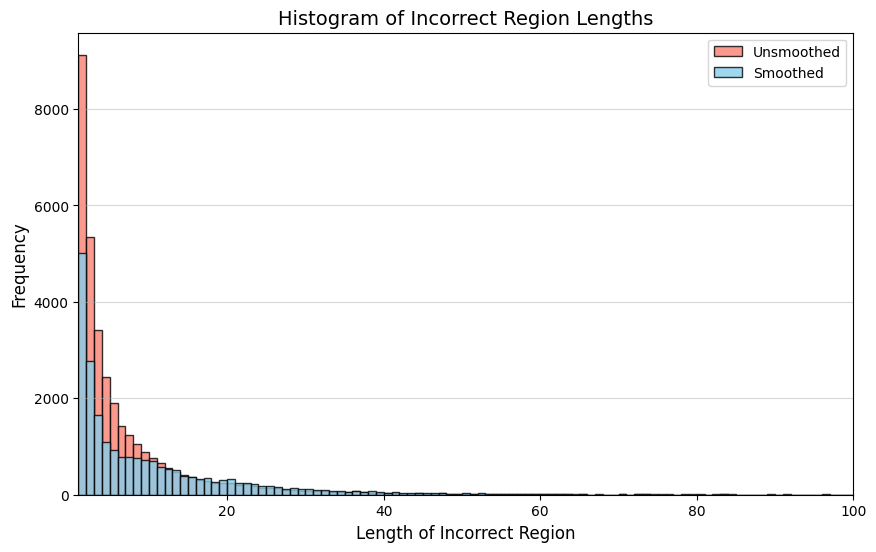
\includegraphics[width=0.6\textwidth]{figures/incorrect_region_smoothing_histogram.png}
    \caption{Histogram over incorrect region lengths for a \emph{CRNN} with and without smoothing. An incorrect region is defined as a sequence if incorrect frames with correct adjacent of either end. Both distributions have a long-tail, with $26.7\%$ regions being of length 1 without smoothing. This raises concerns over the smoothness of outputs and requires some form of post-processing explored in Section~\ref{sec:decoding}. The distribution is more uniform with smoothing, with approximately half the very short incorrect regions.}
    \label{fig:histogram_over_region_lengths}
\end{figure}

\section{Accuracy over the Context}\label{app:accuracy_over_context}
\begin{figure}[H]
    \centering
    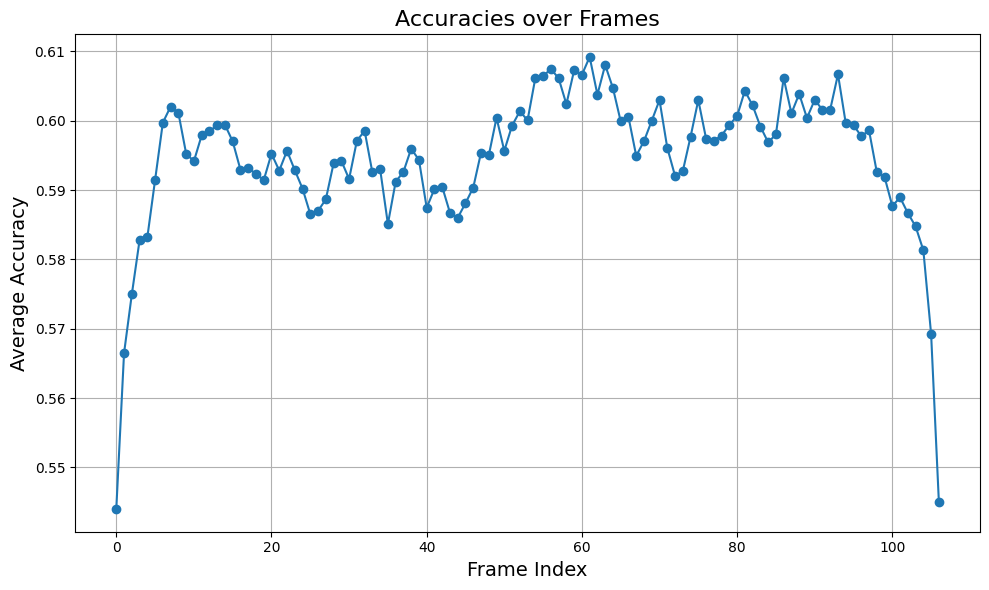
\includegraphics[width=0.8\textwidth]{figures/accuracy_over_frames.png}
    \caption{Average frame-wise accuracy of the \emph{CRNN} model over the patch of audio. The model performs worse at the beginning and end of the patch of audio, as expected. However, the differences are only $~0.05$. We propose that the context on one side is enough for the model to attain the vast majority of the performance attained with bi-directional context. This plot supports our procedure of evaluating over the entire song at once. }\label{fig:crnn_context}
\end{figure}

\section{Accuracy vs Context Length of Evaluation}\label{app:accuracy_vs_context_length}

\begin{figure}[H]
    \centering
    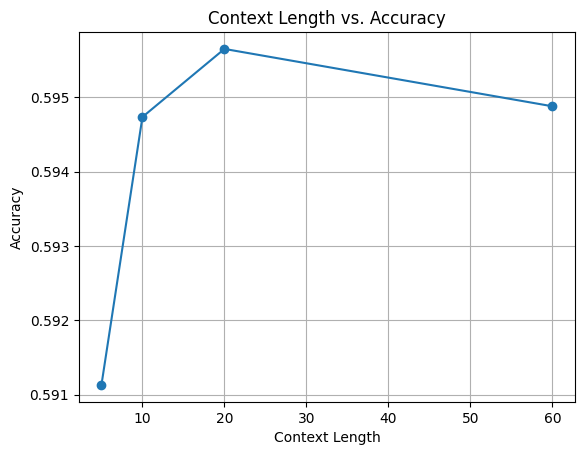
\includegraphics[width=0.5\textwidth]{figures/context_length_vs_accuracy.png}
    \caption{Accuracy with increasing segment length of validation set. The accuracy increases very slightly. I choose to continue evaluating over the entire song at once.}
    \label{fig:accuracy_vs_context_length}
\end{figure}

\section{HMM Smoothing Effect}\label{app:hmm_smoothing_effect}

\begin{figure}[H]
    \centering
    \hspace{-1.5cm}
    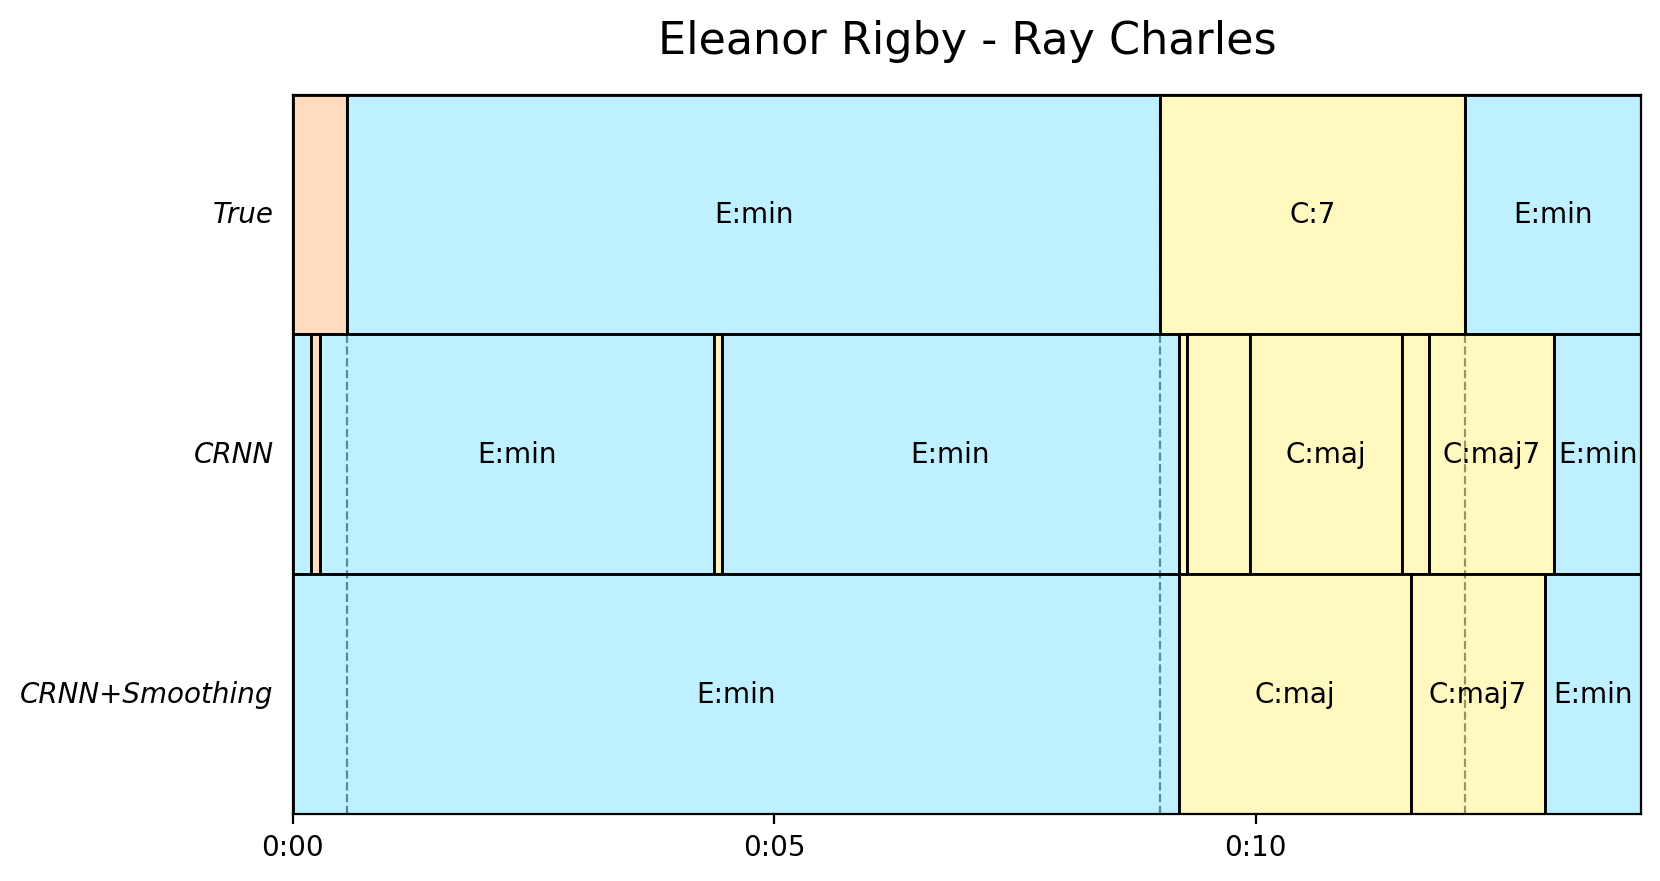
\includegraphics[width=0.9\textwidth]{figures/hmm_smoothing_example.png}
    \caption{An example of the effect of the HMM on the predictions of the \emph{CRNN} model. The top plot shows the ground truth. The middle plot shows frame-wise predictions of the \emph{CRNN} without smoothing. The bottom plot shows the predictions after smoothing. Chords are coloured by their equivalent chord in the small vocabulary as it makes the plot easier to interpret. The original predictions contain many unnecessary and nonsensical chord transitions. These have been smoothed out by the HMM. The resulting chords appear more similar to the ground truth even if frame-wise accuracy has not changed much.}\label{fig:hmm_smoothing_example}
\end{figure}

\section{Weighted Loss Confusion MAtrix}\label{app:weighted_loss_confusion_matrix}

\begin{figure}[H]
    \centering
    \hspace{-1.5cm}
    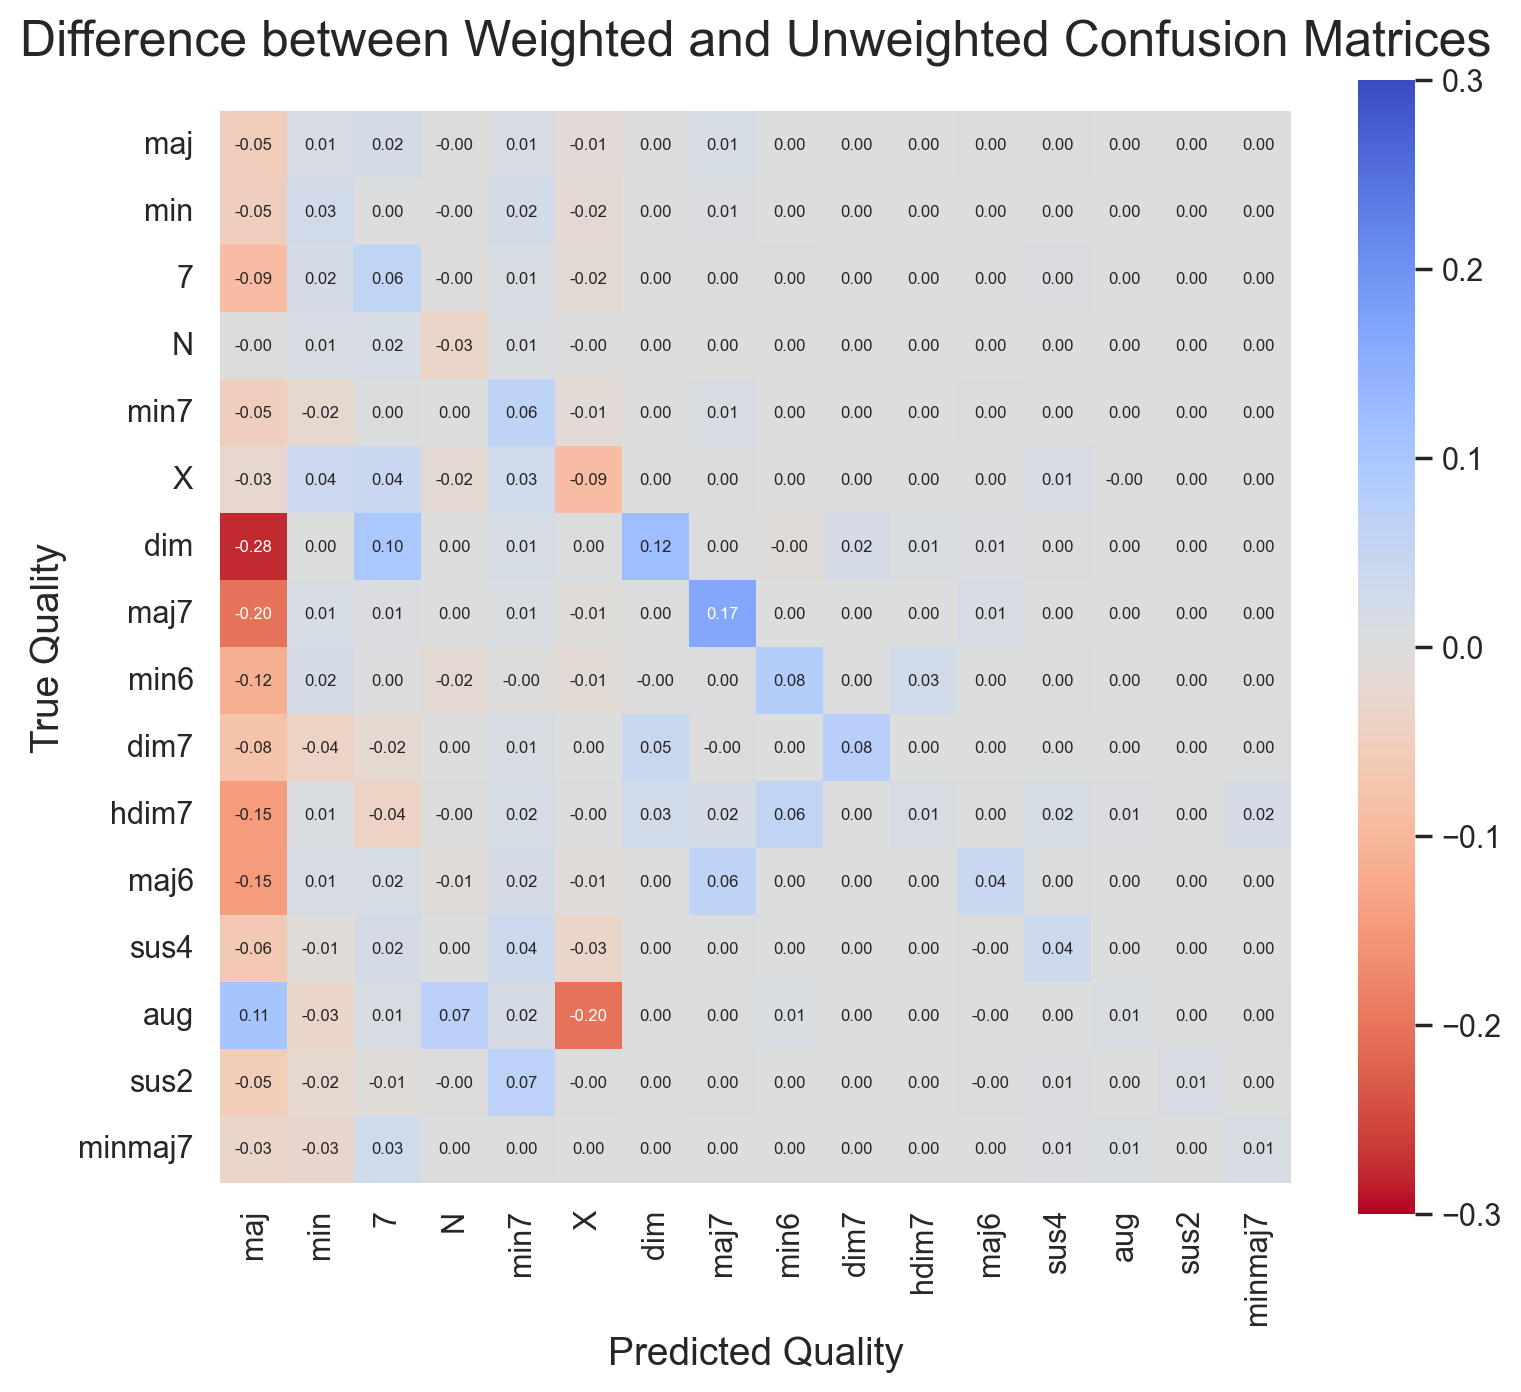
\includegraphics[width=0.9\textwidth]{figures/confusion_matrix_difference.png}
    \caption{ Most of the diagonal entries in the confusion matrix increase. Recall on major7 qualities increases by $0.17$. The only qualities to decrease in recall are major, \texttt{N} and \texttt{X}. I conclude that weighting the loss does improve the model. The weighted model predicts \texttt{X} $2.2$ times less often. This may be how the weighted model improves class-wise metrics without sacrificing too much overall accuracy since \texttt{X} frames are ignored for evaluation.}\label{fig:hmm_smoothing_example}
\end{figure}

\section{Details of Generative Feature Extraction}\label{app:generative_feature_extraction}

\section{Upsampling Methods in Generative Feature Extraction}\label{app:linear_interpolation_vs_area_averaging}

\begin{table}[H]
    \centering
    \begin{tabular}{cccccc}
        \toprule
        upsample & accuracy & root & third & seventh & mirex  \\  
        \midrule
        area & \textbf{59.4} & \textbf{77.8} & \textbf{74.6} & \textbf{61.7} & \textbf{78.1} \\
        lerp & 58.4 & 77.7 & 74.0 & 60.6 & 78.2 \\
        \bottomrule
    \end{tabular}
    \caption{Comparison of generative feature extraction with linear interpolation and area averaging for the musicgen-large and a linear projection down to $64$ dimensions and averaging over the four codebooks. The results are very similar, but the area averaging method is slightly better in all metrics. I therefore choose to continue averaging over model frames in order to upsample to CQT frames.}\label{tab:linear_interpolation_vs_area_averaging}
\end{table}

\section{Generative Feature Low-Dimensional Projection}\label{app:projection_dimensionality}

\begin{table}[H]
    \centering
    \begin{tabular}{cccccc}
        \toprule
        $d$ & accuracy & root & third & seventh & mirex  \\  
        \midrule
        16   & 58.4       & 77.6       & \textbf{74.5} & 60.6       & 77.2       \\
        32   & 57.8       & 77.5       & 73.6          & 60.0       & 77.8       \\
        64   & \textbf{59.2} & 77.5    & 74.3          & \textbf{61.4} & \textbf{77.9} \\
        128  & 58.1       & 77.0       & 73.6          & 60.3       & 77.4       \\
        256  & 58.7       & 77.6       & 74.3          & 60.9       & 77.5       \\
        512  & 58.3       & \textbf{77.9} & 74.3      & 60.6       & 77.6       \\
        1024 & 58.4       & 76.7       & 73.5          & 60.7       & 76.7       \\ 
        \bottomrule
    \end{tabular}
    \caption{Generative feature extraction with different projection dimensions, $d$. All results use the musicgen-large model and average across the four codebooks. There are no large differences between the different dimension reductions. I take $d=64$ as it performs the best, but there is no evidence that this is not due to randomness in the optimisation process. }\label{tab:projection_dimensionality}
\end{table}

\section{Generative Features with Different Models}\label{app:generative_feature_extraction_models}

\begin{table}[H]
    \centering
    \begin{tabular}{lc}
        \toprule
        model  & acc  \\
        \midrule
        large  & \textbf{60.2} \\
        small  & 59.8 \\
        melody & 59.9 \\
        chord  & 59.7 \\
        \bottomrule
    \end{tabular}
    \caption{Results for generative features extracted from MusicGen~\citep{MusicGen} and MusiConGen~\citep{MusiConGen} models with different musicgen-models. Only accuracy is reported as the other metrics are qually similar. These models are musicgen-large, musicgen-small, musicgen-melody and MusiConGen, referred to as large, small, melody and chord respectively. There are very few differences between the models. This suggests that the small model has just as much information in its internal representations that is useful for identifying chords as the other models. Another point of note is the comparison between chord and melody. The chord model is a chord-conditioned fine-tuned version of melody. It is surprising that the chord-conditioning did not help compared to the non chord-conditioned model.}\label{tab:musicgen_pivot}
\end{table}

\section{Generative Features with Different Codebook Reductions}\label{app:generative_feature_extraction_reductions}

\begin{table}[H]
    \centering
    \begin{tabular}{lc}
        \toprule
        reduction   & accuracy \\  
        \midrule
        concat       & 58.9     \\
        codebook\_2  & 58.9     \\
        codebook\_3  & 57.5     \\
        codebook\_1  & 59.0     \\
        codebook\_0  & 58.1     \\
        avg          & \textbf{59.4}     \\
        \bottomrule
    \end{tabular}
    \caption{Accuracy for different codebook reduction methods. Other metrics are omitted as they do not provide more information. All results are for musicgen-large with reduction down to $64$ dimensions. Reductions of the form `codebook\_$n$' refer to training on codebook of index $n$ from the model. Performance is similar across reductions except for codebook\_0 and codebook\_3 which perform worse. I choose the averaging reduction based on maximum accuracy. }\label{tab:reduction_accuracy}
\end{table}
